\documentclass{scrartcl}

\KOMAoptions{
	paper=a4,
	fontsize=12pt,
	parskip=true,
	titlepage=false,
	toc=bibliography,
	%abstract=true,
}
%\KOMAoption{toc}{bibliography}

\addtokomafont{disposition}{\boldmath}

% section numbering
%\renewcommand*{\thesection}{\thepart.\arabic{section}}
%\DeclareTOCStyleEntry[numwidth=0.85cm]{tocline}{section}

\usepackage{fontspec}
\setmainfont{Free Serif}
\setsansfont{Free Sans}
% URLs should (still) be typed using monospace font
% https://graphicdesign.stackexchange.com/questions/97173/is-monospacing-urls-in-academic-papers-still-advised
\setmonofont{inconsolata}
%\newfontfamily\DejaSans{DejaVu Sans} % to display emojis

\usepackage{csquotes} % quotation marks
\usepackage[onehalfspacing]{setspace}
\usepackage{mathtools}
\usepackage[english]{translator} % siunitx needs translator package (not ngerman)! 
\usepackage{siunitx}[=v2]
\sisetup{%
	separate-uncertainty=true,
	locale=UK,
	range-units=single,
	%mode=match
	%per-mode=fraction,
}
\DeclareSIUnit\ppm{\text{ppm}}
\DeclareSIUnit\year{\text{yr}}
\NewDocumentCommand{\angsi}{omom}{%
	\ang[#1]{#2}\,\si[#3]{#4}%
}
% https://tex.stackexchange.com/questions/116426/recommend-way-to-get-angular-velocity-in-degree-with-siunitx
\usepackage[
pdfauthor={Robert Wright},
%pdftitle={},
]{hyperref}
\hypersetup{
	colorlinks=true,
	urlcolor=cyan,
	linkcolor=,
	citecolor=,
}

\usepackage{graphicx}
	% Placing float (table or figure) at the top of the page in otherwise empty page
	\makeatletter
	\setlength\@fptop{0\p@}
	\makeatother
\usepackage[verbose]{wrapfig} % figure and text side-by-side
\usepackage{float}
\usepackage{pdfpages}
\usepackage{caption}
\usepackage{subcaption}
\usepackage{cleveref}
\usepackage{booktabs}
\usepackage{tabularx} % automatic line breaks in tables
	% redefine the X column to be based on a m-column instead of a p-column
	\renewcommand\tabularxcolumn[1]{m{#1}} 
\usepackage{multirow, makecell}
\usepackage[roman]{parnotes}
\usepackage[shortcuts]{extdash} % to hyphenate words with dashes in them
\usepackage{xcolor}
%\usepackage[enable]{easy-todo}
\usepackage[version=4]{mhchem}

% LANGUAGE & DATE
% Note: In general, it is advisable to activate the languages
%       after all packages have been loaded
\usepackage{polyglossia}
	\setdefaultlanguage[variant=british]{english}
% load datetime2 after language is set
% (can’t detect the region with polyglossia)
\usepackage[en-GB]{datetime2}
	\DTMlangsetup[en-GB]{ord=raise}

% REFERENCES
\usepackage[
	backend=biber,
	style=numeric-comp,
	sorting=none,
	%bibstyle=authortitle,
	autolang=langname,
	uniquename=init,
	giveninits=true,
	maxnames=2,
	% sets the option for all dates to the same value
	alldates=terse,
	%block=ragged,
]{biblatex}
\addbibresource{../../literature/glaciology.bib}
% don't print url and urldate
%\AtEveryBibitem{
%	\clearfield{url}
%	\clearfield{urlyear}
%}

%%%%%%%%%%%%%%%%%%%%%%%%%%%%%%%%%%%%%%%%%%%%%%%%%%%%%%%%%%%%%%%%%%%%%%%%%%%%%%%%%%%
% https://tex.stackexchange.com/questions/16765/biblatex-author-year-square-brackets
\makeatletter

\newrobustcmd*{\parentexttrack}[1]{%
	\begingroup
	\blx@blxinit
	\blx@setsfcodes
	\blx@bibopenparen#1\blx@bibcloseparen
	\endgroup}

\AtEveryCite{%
	\let\parentext=\parentexttrack%
	\let\bibopenparen=\bibopenbracket%
	\let\bibcloseparen=\bibclosebracket}

\makeatother
%%%%%%%%%%%%%%%%%%%%%%%%%%%%%%%%%%%%%%%%%%%%%%%%%%%%%%%%%%%%%%%%%%%%%%%%%%%%%%%%%%%
% COSTUM COMMANDS

% change figsize globally
\newcommand{\figwidth}{0.9\linewidth}

\newcommand{\kopf}[1]{%
	\Large\textsf{\textbf{#1}}
}

% Markdown code style
\definecolor{light-gray}{gray}{0.95}
\newcommand{\code}[1]{\colorbox{light-gray}{\texttt{#1}}}

% math stuff
\newcommand*\mean[1]{\overline{#1}}
\newcommand{\vect}[1]{\boldsymbol{#1}}

% chemnistry stuff
\newcommand{\co}{\ce{CO2}}

%%%%%%%%%%%%%%%%%%%%%%%%%%%%%%%%%%%%%%%%%%%%%%%%%%%%%%%%%%%%%%%%%%%%%%%%%%%%%%%%%%%
% TITLE

\subject{GEOV325: Glaciology}
\title{Simulating the Greenland Ice Sheet}
\subtitle{Using a Two-Dimensional Ice Flow Model}
\author{Robert Wright}
\publishers{University of Bergen}
\date{\DTMdisplaydate{2024}{6}{14}{-1}}

%%%%%%%%%%%%%%%%%%%%%%%%%%%%%%%%%%%%%%%%%%%%%%%%%%%%%%%%%%%%%%%%%%%%%%%%%%%%%%%%%%%

\begin{document}
	
	\maketitle
	\tableofcontents 
	% https://tex.stackexchange.com/questions/341613/komascript-toc-prevent-column-break-between-sections-in-multicolumn-toc
	
	%\input{sections/abstract.tex}
	\section{Introduction}

% TODO:
% - Datum auf erster Seite richtig anzeigen
% - Wie binde ich den Abstract ein?
% - Foto auf Titelseite?

% Please write an individual report about the field work at Folgefonna of about 2000 words. Since we did not spend a lot of time in the field and have limited data, the focus should be the process of data retrieval, how to prepare and log measurements, dealing with the imperfections of field work, and a discussion of how these challenges affect data quality.

% https://advice.writing.utoronto.ca/types-of-writing/lab-report/

% Introduction and motivation (Why are we interested in field data from Folgefonna?)

Folgefonna is a glacier in Norway.

\subsection{Theoretical Background}
	\section{The Greenland ice sheet model}

% Is the model set up correctly, i.e., as per instructions and without coding errors? (10 points)
% Is the performance of the model sufficiently documented with figures and (quantified) analysis? At least one figure showing the ice thickness should be shown, and one section through the ice sheet. (5 points)
% Discuss if the model is producing accurate results. Why do you trust it? (5 points)

The GrIS is simulated using a two-dimensional ice flow model. Generally speaking, ice flow is driven by hydrostatic pressure exerting differential shear stress due to variations in glacier height. Glen's flow law, an empirical relation between strain rate and stress, allows to derive the vertically-integrated velocity
\begin{equation}\label{eq:meanu}
\mean{u} = -\frac{2}{5}A \left( \rho g \delta_x z \right)^3 h^4,	
\end{equation}
where \(A\) is the so-called flow parameter, \(\rho\) the ice density, \(g\) the gravitational acceleration, \(z\) the surface elevation, and \(h\) the ice thickness. 
\Cref{eq:meanu} can be extended to an ice flux \(F\), which in turn, combined with the surface mass balance  \(M\) (i.e., the net balance of accumulation and ablation) yields the change of ice thickness in time 
\begin{equation}\label{eq:flux}
	\delta_t h = -\nabla F + M = -\nabla (\mean{u}h) + M.
\end{equation}

\subsection{Benchmarking}

In order to initially verify the ice flow model, a benchmark simulation spanning \SI{10000}{\year} is performed. The spatial domain of this simulation (like all others) has a resolution of \SI{40}{\km}. It is run on flat bedrock, paired with an artificial surface mass balance (SMB). Inside a 10\(\times\)10 grid box the SMB is positive (\(M = \SI{2}{\m\per\year}\)), while outside this area \(M = \SI{-2}{\m\per\year}\) is applied. \Cref{fig:benchmark-map} indirectly illustrates the benchmark SMB in the upper-left subplot, since the growing ice thickness matches the area of positive SMB. On top, we observe that the expansion of the ice ultimately reaches an equilibrium in the shape of a circle with maximum ice thickness at its centre. 

\begin{figure}
	\centering
	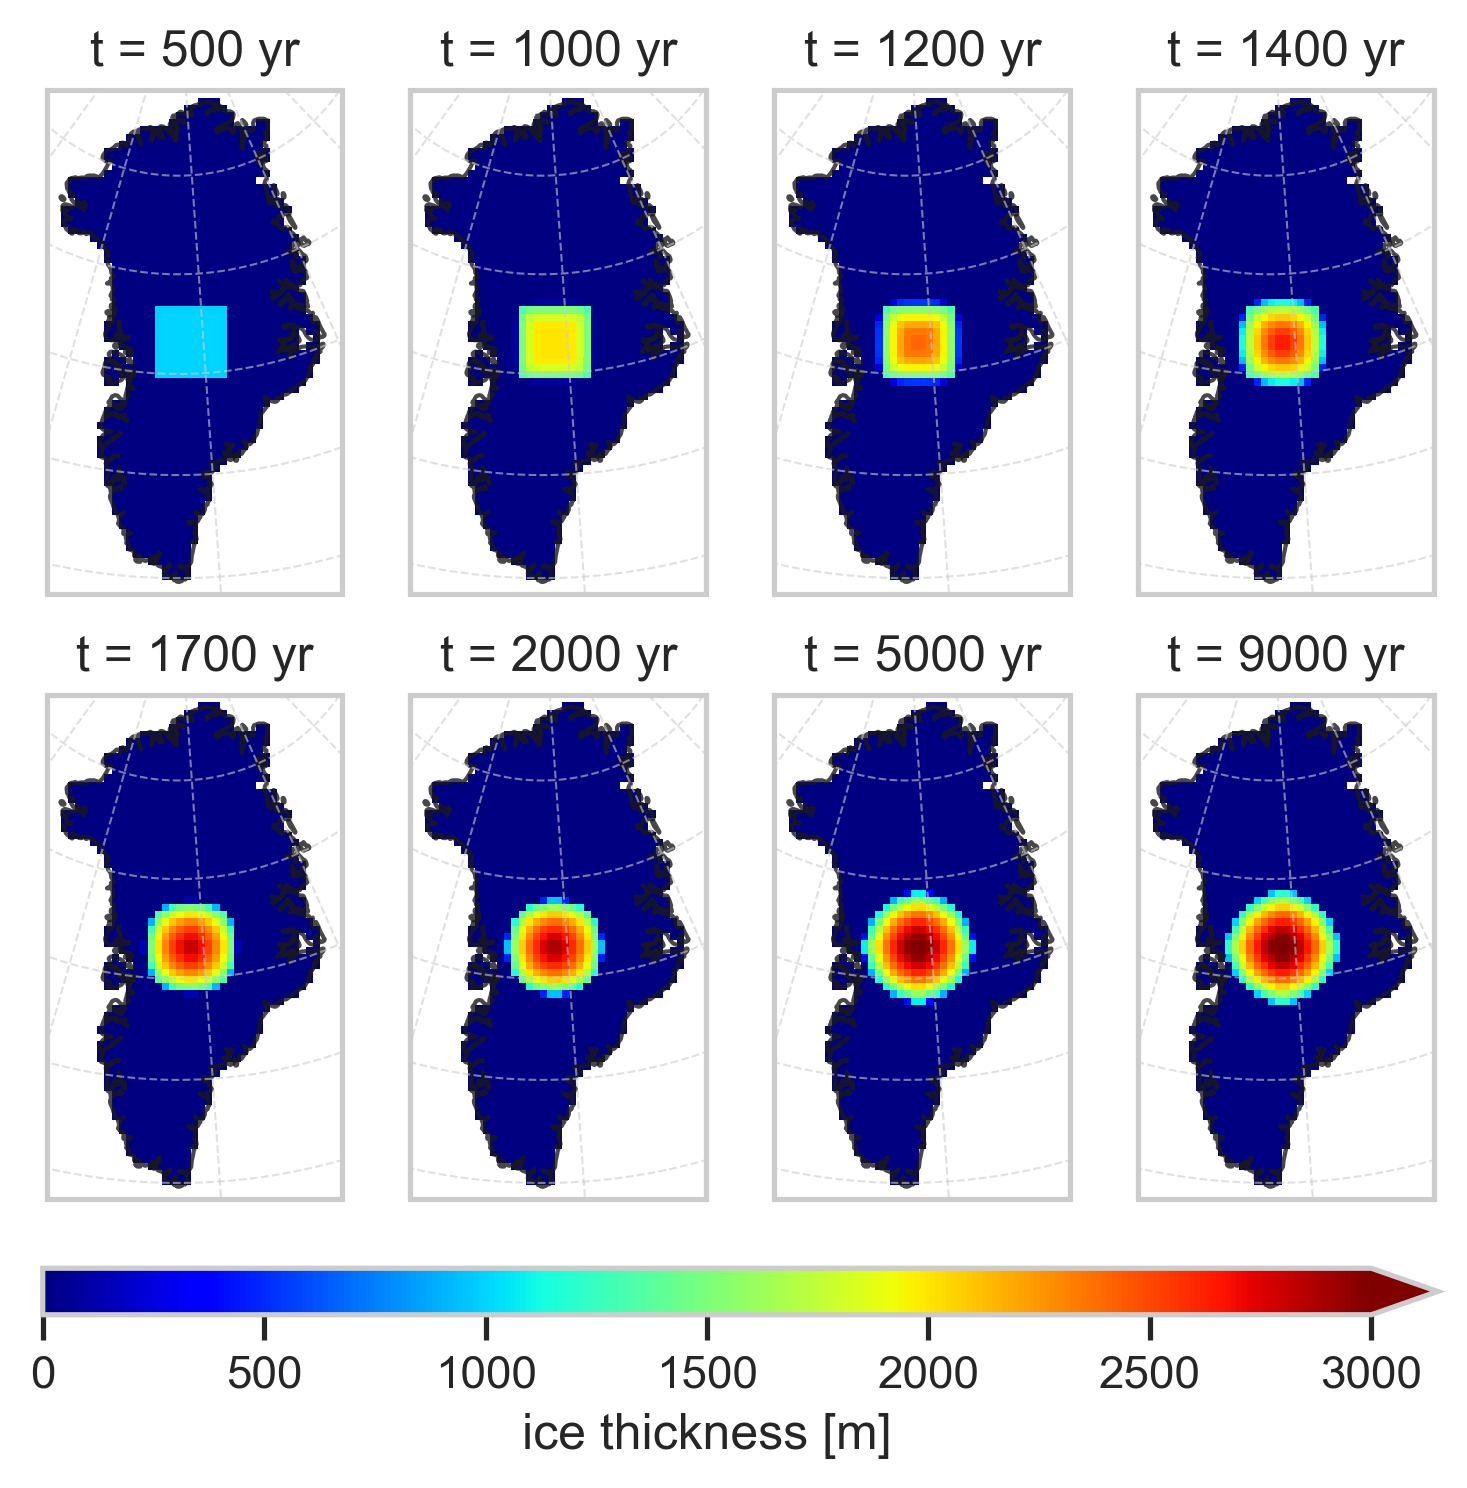
\includegraphics[width=0.7\linewidth]{../benchmark/figs/ice-map.png}
	\caption{Map of ice thickness at time steps \(t\) during the benchmark simulation}
	\label{fig:benchmark-map}
\end{figure}

\begin{figure}
	\centering
	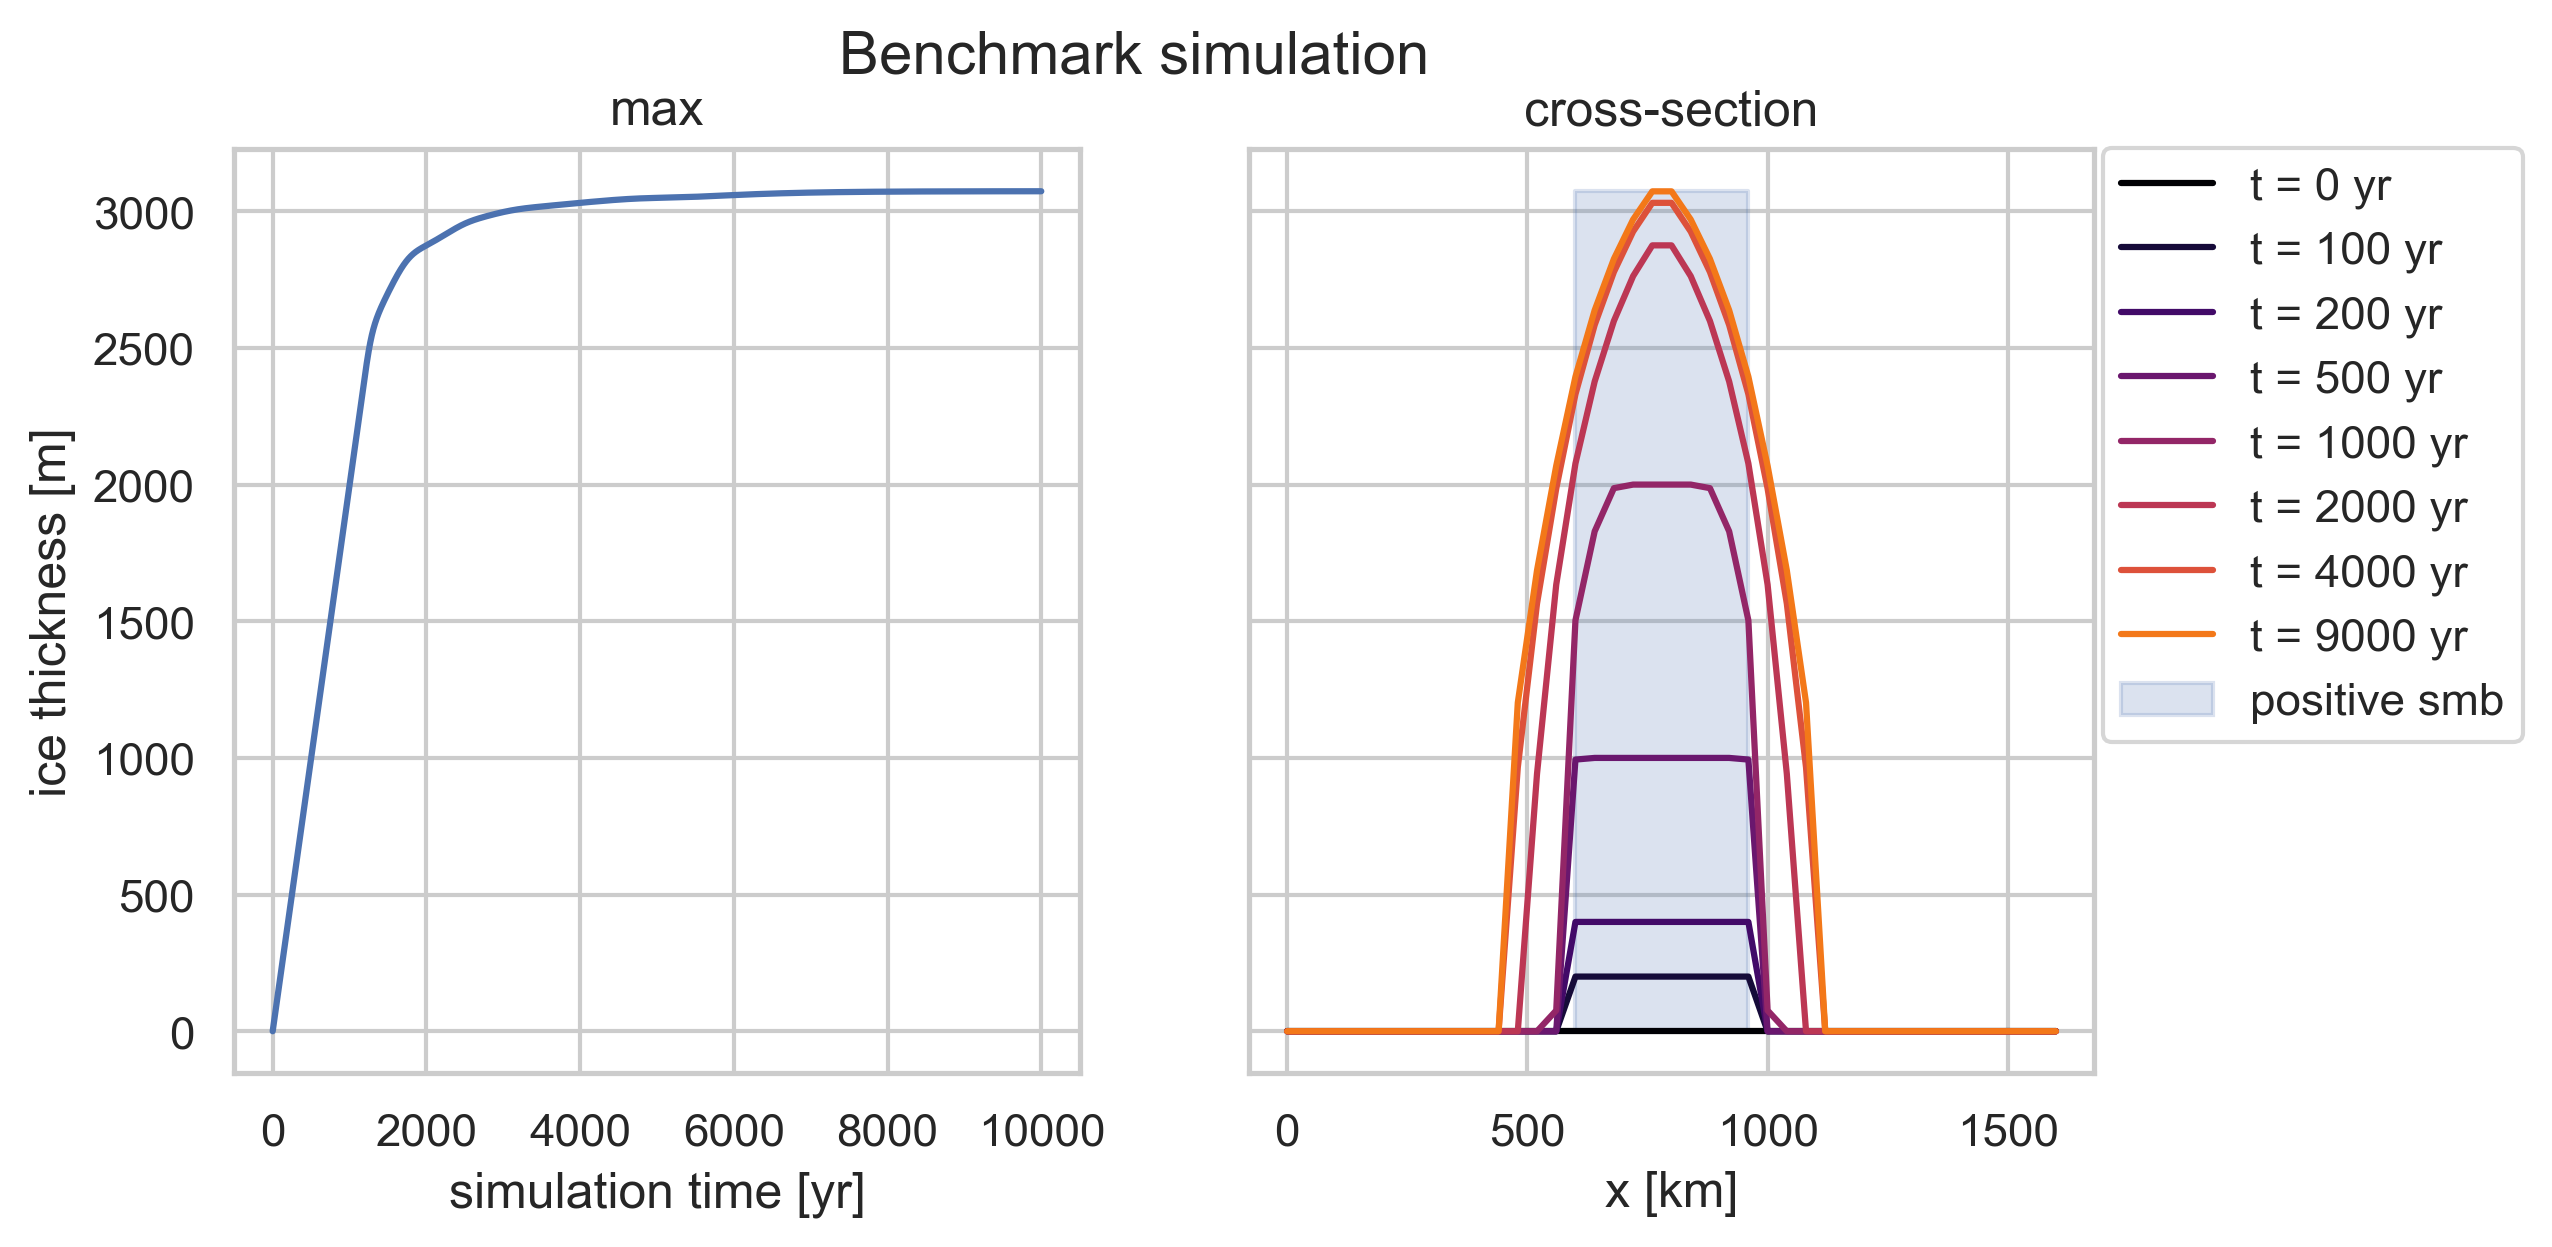
\includegraphics[width=\linewidth]{../benchmark/figs/cross-section.png}
	\caption{\textit{Left:} Maximum ice thickness throughout simulated years. \textit{Right:} West-east cross-section of ice thickness; the region of positive SMB is found in-between the dashed lines.}
	\label{fig:benchmark-cross-section}
\end{figure}

The equilibrium state is characterized by a maximum ice thickness of just over \SI{3000}{\m} after approximately \SI{4000}{\year} of simulation  (\cref{fig:benchmark-cross-section}). The ice flow becomes increasingly noticeable from \SI{1000}{\year} onwards, after an ice thickness of around \SI{2000}{\m} has been reached. From \(F \propto h^5\) in \cref{eq:flux} it is to be expected that a certain height has to be reached before considerable ice flow can occur. Qualitatively, the isotropic flow and shape of the ice sheet is comparable to the results of other students and the benchmark data agrees well with what has been mentioned in the (video) lectures.

\subsection{Surface mass balance}\label{sec:smb}

After benchmarking the simulation, the upcoming model runs feature a more realistic SMB. The annual melting \(\mathrm{M}\) of the ice sheet is derived from an artificial temperature field \(T\) using a positive degree day approach
\begin{equation}\label{eq:melt}
	\mathrm{M} = \beta \cdot \sum_{i=\mathrm{Jan\, 1}}^{\mathrm{Dec\, 31}} \max \left(T_{i},\SI{0}{\celsius}\right),
\end{equation}
while the accumulation \(\mathrm{A}\) is simplified to all precipitation \(P\) at temperatures below the freezing point 
\begin{equation}\label{eq:acc}
	\text{A} = \sum_{i=\mathrm{Jan\, 1}}^{\mathrm{Dec\, 31}}P_{i},\quad \text{if}\ T_i < \SI{0}{\celsius}.
\end{equation}
Combined, \cref{eq:melt,,eq:acc} yield the annual SMB in \si{\mm\per\year}. The melting factor \(\beta\) relates melting and accumulation (it also ensures that the SMB has the correct units) and is set to \(\beta = \SI{5}{\mm\per\day\per\celsius}\) as this is within the interval of the ice and snow melting factor used by \textcite{seguinot2013}. 

\begin{table}
	\centering
	\begin{tabularx}{\textwidth}{llX}
		\toprule
		Variable & Mechanism & Scaling factor \\
		\midrule
		Temperature & Linear latitudinal gradient & North-south difference: \SI{15}{\celsius} \\
		 & Elevation & Lapse rate: \SI{0.65}{\celsius}\(/\)\SI{100}{\m} \\
		 & Seasonality & Cosine function; winter-summer difference: \SI{20}{\celsius} \\
		 & Weather & Normal distribution; standard deviation: \SI{3.5}{\celsius} \\
		\midrule
		Precipitation & Linear latitudinal gradient & North-south difference: \SI{6}{\mm\per\day} \\
		 & Euclidean distance to coastline & \(\left[\left(0.1 \cdot \text{distance[\# grid points]}\right)+1\right]^{-1}\) \\
		\bottomrule
	\end{tabularx}
	\caption{Considered scaling processes to initialize temperature and precipitation fields}
	\label{tab:smb}
\end{table}

The artificial temperature and precipitation fields are scaled by multiple processes presented in \cref{tab:smb}, the individual scaling factors are chosen to (roughly) match the reanalysis data in \cref{app:era5}. To further confirm the choice and magnitude of the scalings, the resulting SMB displayed in \cref{fig:smb-ref} is qualitatively compared to modelled SMB maps by \textcite{fettweis2020}.

\begin{figure}[H]
	\centering
	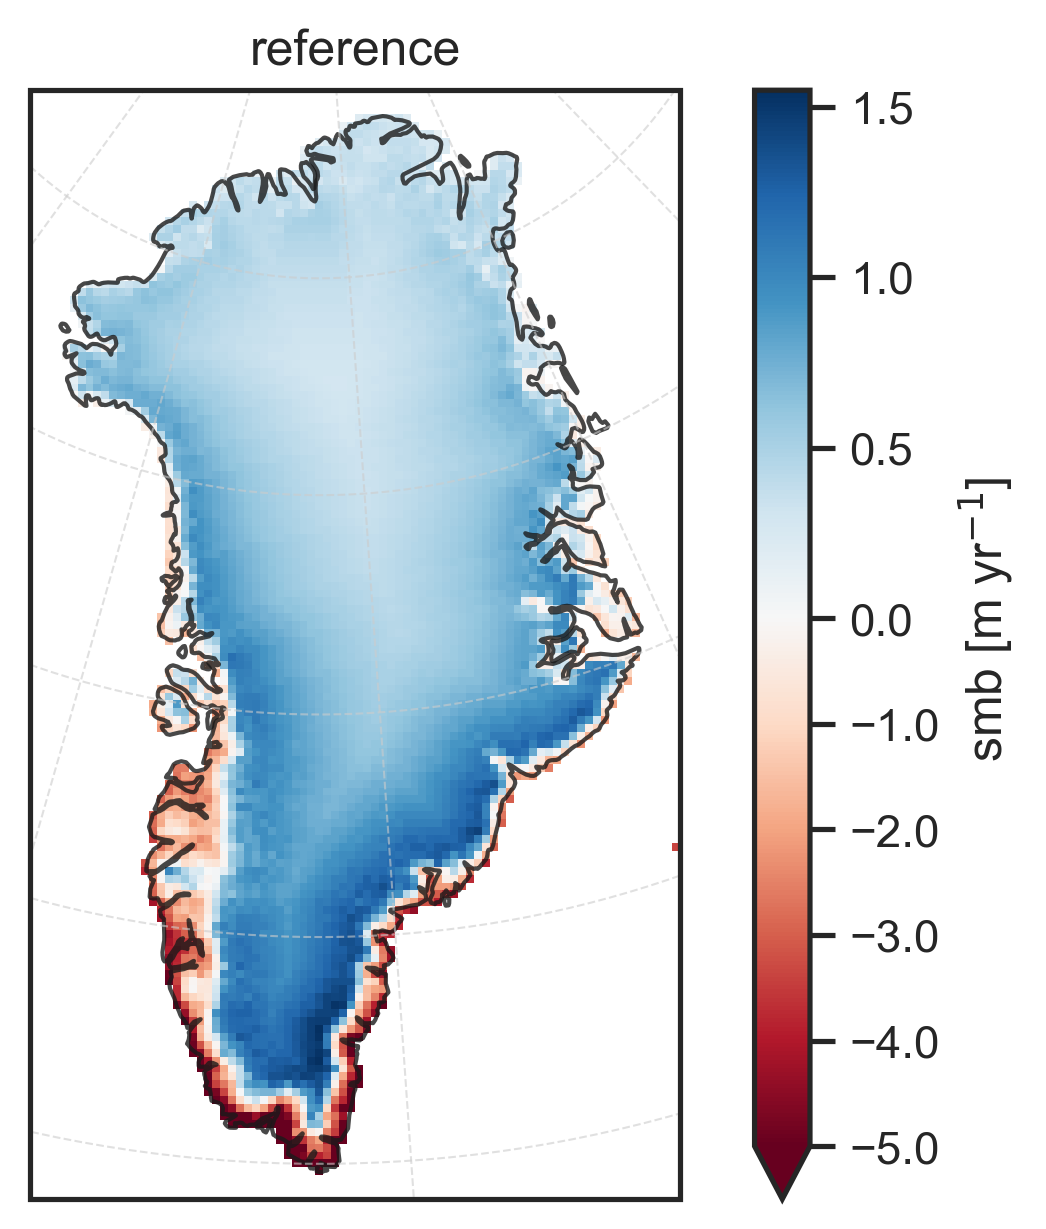
\includegraphics[width=0.45\textwidth]{../../climate-change-scenarios/smb-map-reference.png}
	\caption{SMB calculated from temperature and precipitation fields based on default scaling factors introduced in \cref{tab:smb}; please note that the colorbar uses a different scaling for positive and negative values.}
	\label{fig:smb-ref}
\end{figure}

	\section{Results}

% Analysis of results (What does the data show? (can be short, use figures))
	\section{Discussion}

% A good report will link the field measurements with what we learned in class and, if possible, published literature. A few guiding questions could be 'Do the observations show what we expected?', 'What could explain a possible disagreement?', and 'If we had more time, how could that improve our data?'. A critical discussion of the shortcomings and advantages of the methodology is also important. 

% Discussion and conclusion (Is the data any good? What could be improved? What would the data look like if we had taken it at a different time of year or at a different elevation?)

% Discussion is the most important part of your report, because here, you show that you understand the experiment beyond the simple level of completing it.


	
	\newpage
	\begingroup
	\hypersetup{urlcolor=.}
	\setlength{\emergencystretch}{3em}
	\printbibliography
	\endgroup
	
	\newpage
	\appendix
	\section{Code availability}\label{app:code}

The two-dimensional ice flow model is written in python and the entire project can be found in an \href{https://gitlab.met.fu-berlin.de/rw0064fu/glaciology}{online repository}\footnote{\hypersetup{urlcolor=}\url{https://gitlab.met.fu-berlin.de/rw0064fu/glaciology}}. The ice transport equations are numerically solved in the main model part found in \code{2d-ice-sheet/2d\_model.py}, while the SMB is externally computed and updated in the \code{2d-ice-sheet/surface\_mass\_balance.py} file. The corresponding parameters for initializing the temperature and precipitation fields are stored in the \code{params.py} files in the respective subdirectories.

\section{SMB parametrization}\label{app:era5}

In order to derive an estimate for the values of the different scaling methods in \cref{tab:smb}, multi-year plots of the mean
temperature (\cref{fig:era5}) and precipitation (\cref{fig:era5-pr}) in Greenland are created based on ERA5 reanalysis data from 2010 to 2019.

\begin{figure}[h]
	\centering
	\begin{subfigure}{0.49\textwidth}
		\centering
		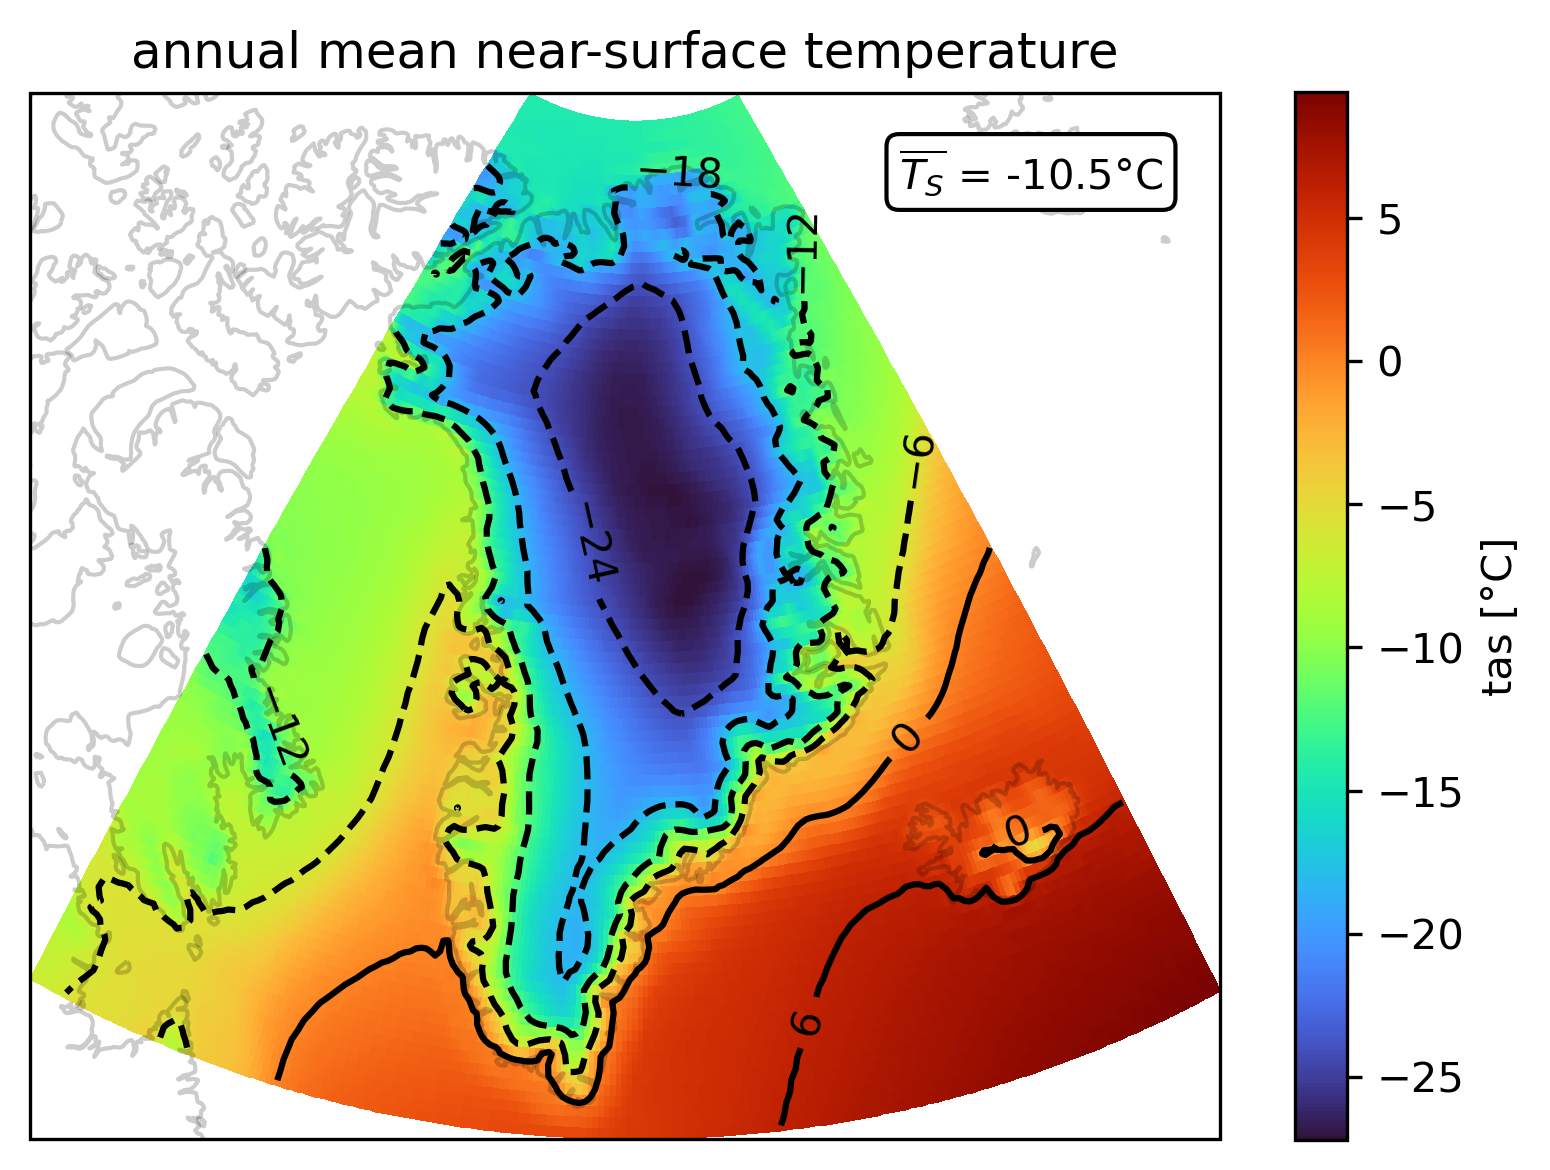
\includegraphics[width=\textwidth]{../../era5/figs/tas-annual-mean.png}
	\end{subfigure}
	\begin{subfigure}{0.49\textwidth}
		\centering
		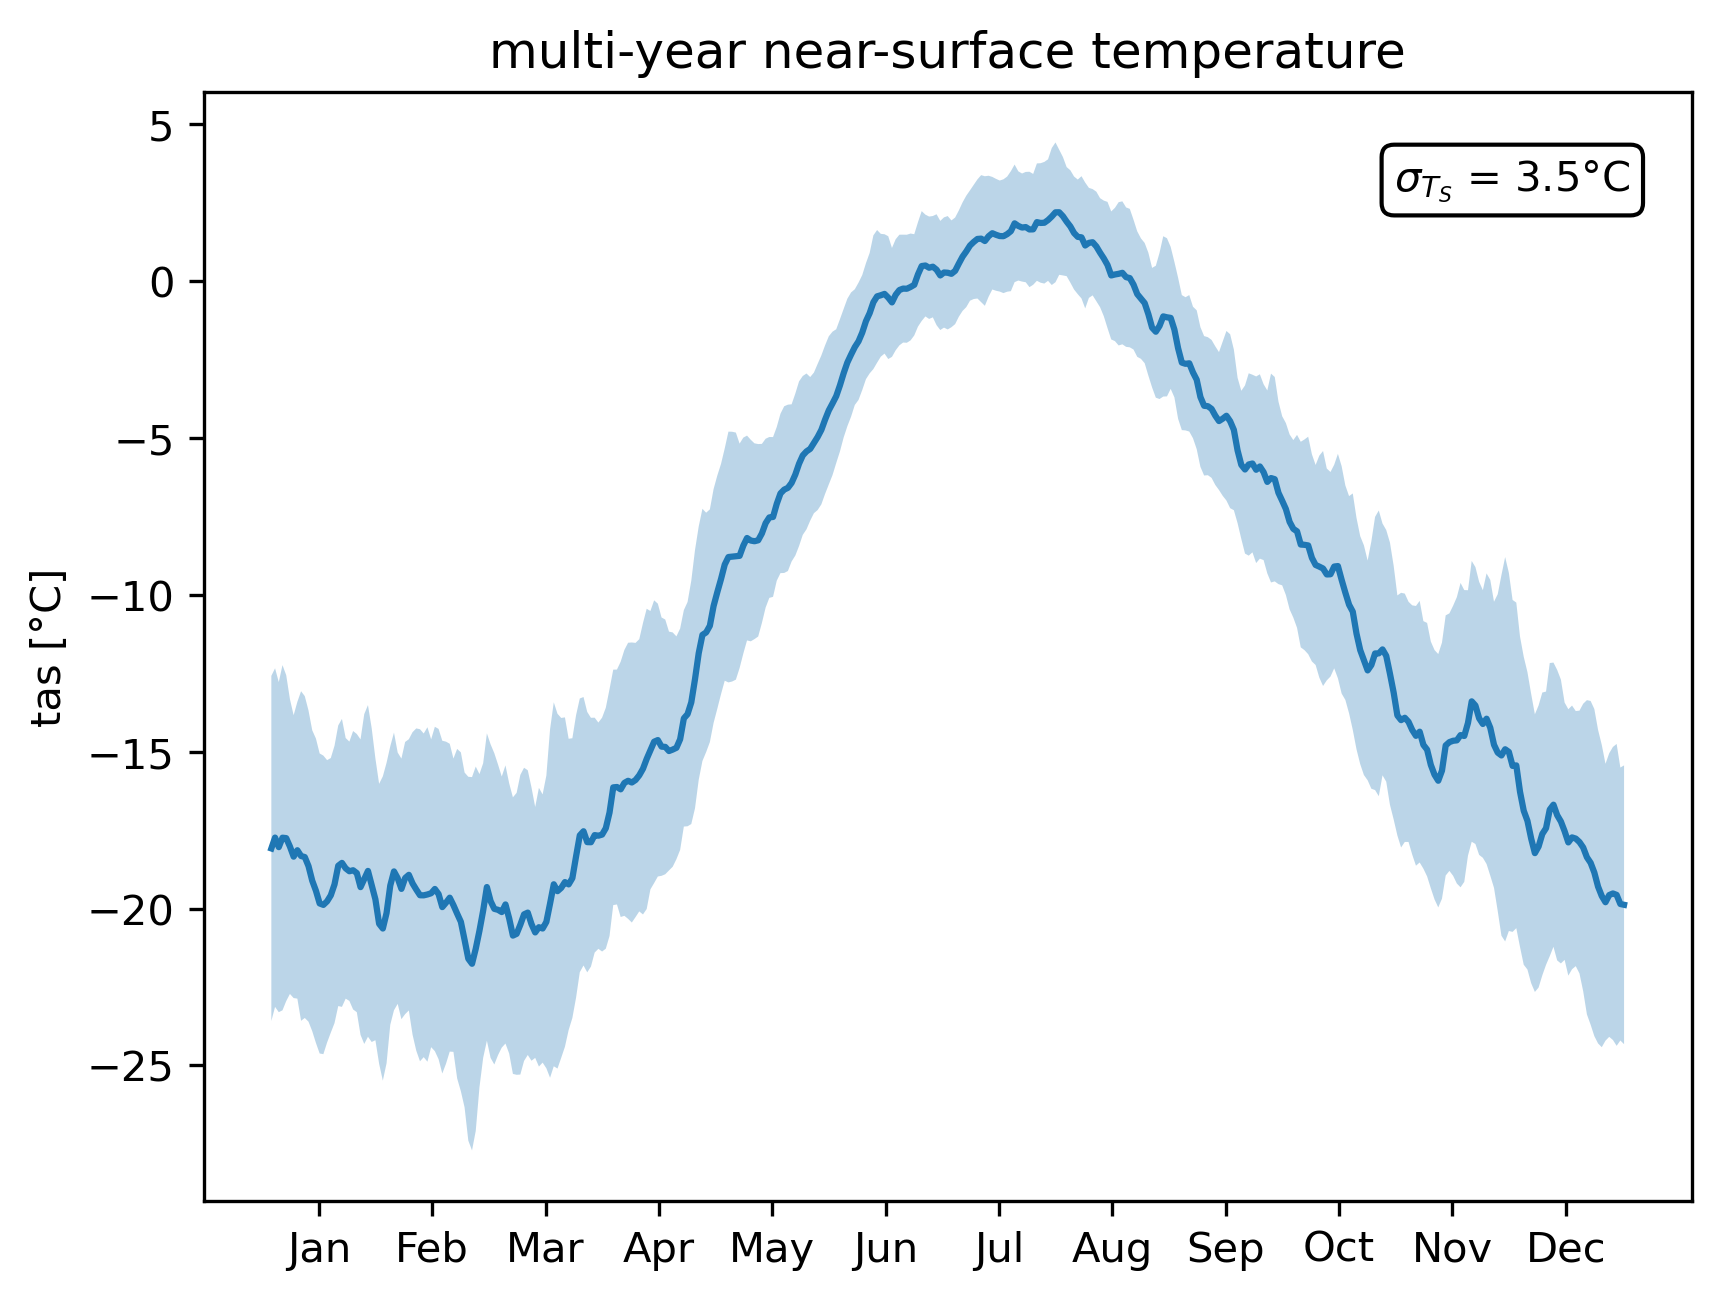
\includegraphics[width=\textwidth]{../../era5/figs/tas-seasonality.png}
	\end{subfigure}
	\caption{Spatial distribution and seasonality of temperature field}
	\label{fig:era5}
\end{figure}

\begin{figure}
	\centering
	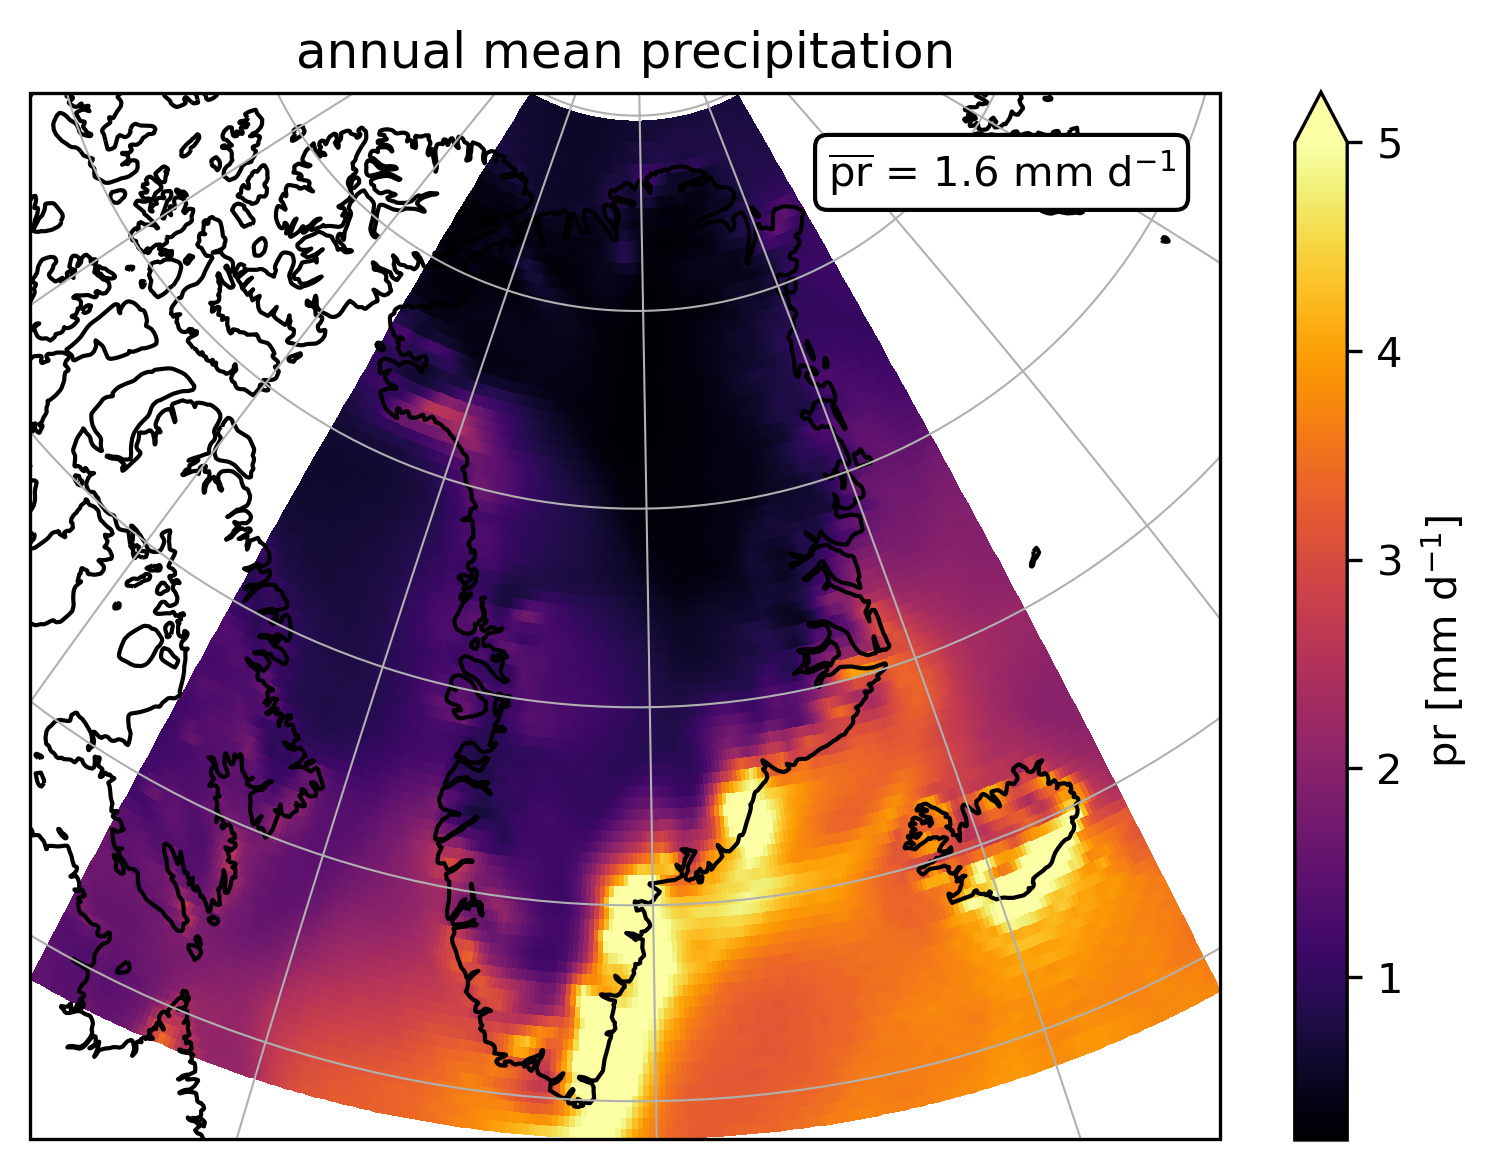
\includegraphics[width=0.6\textwidth]{../../era5/figs/pr-annual-mean.png}
	\caption{Precipitation field; the maximum annual precipitation is \(\mean{P}_{\text{max}} = \SI{8.84}{\mm\per\day}\) (not displayed by cropped colorbar)}
	\label{fig:era5-pr}
\end{figure}

\section{Climate forcings}

\subsection{NorESM}\label{app:forcing-noresm}

The NorESM climate forcing depends on a future projection of the climatology, scaled by a climate index (\cref{fig:climate-index}) to match the respective year of the simulation. For roughly the first \SI{200}{\year}, the climate index increases, until reaching a constant value of \(\approx\num{3}\) for the remaining time.  

\begin{figure}
	\centering
	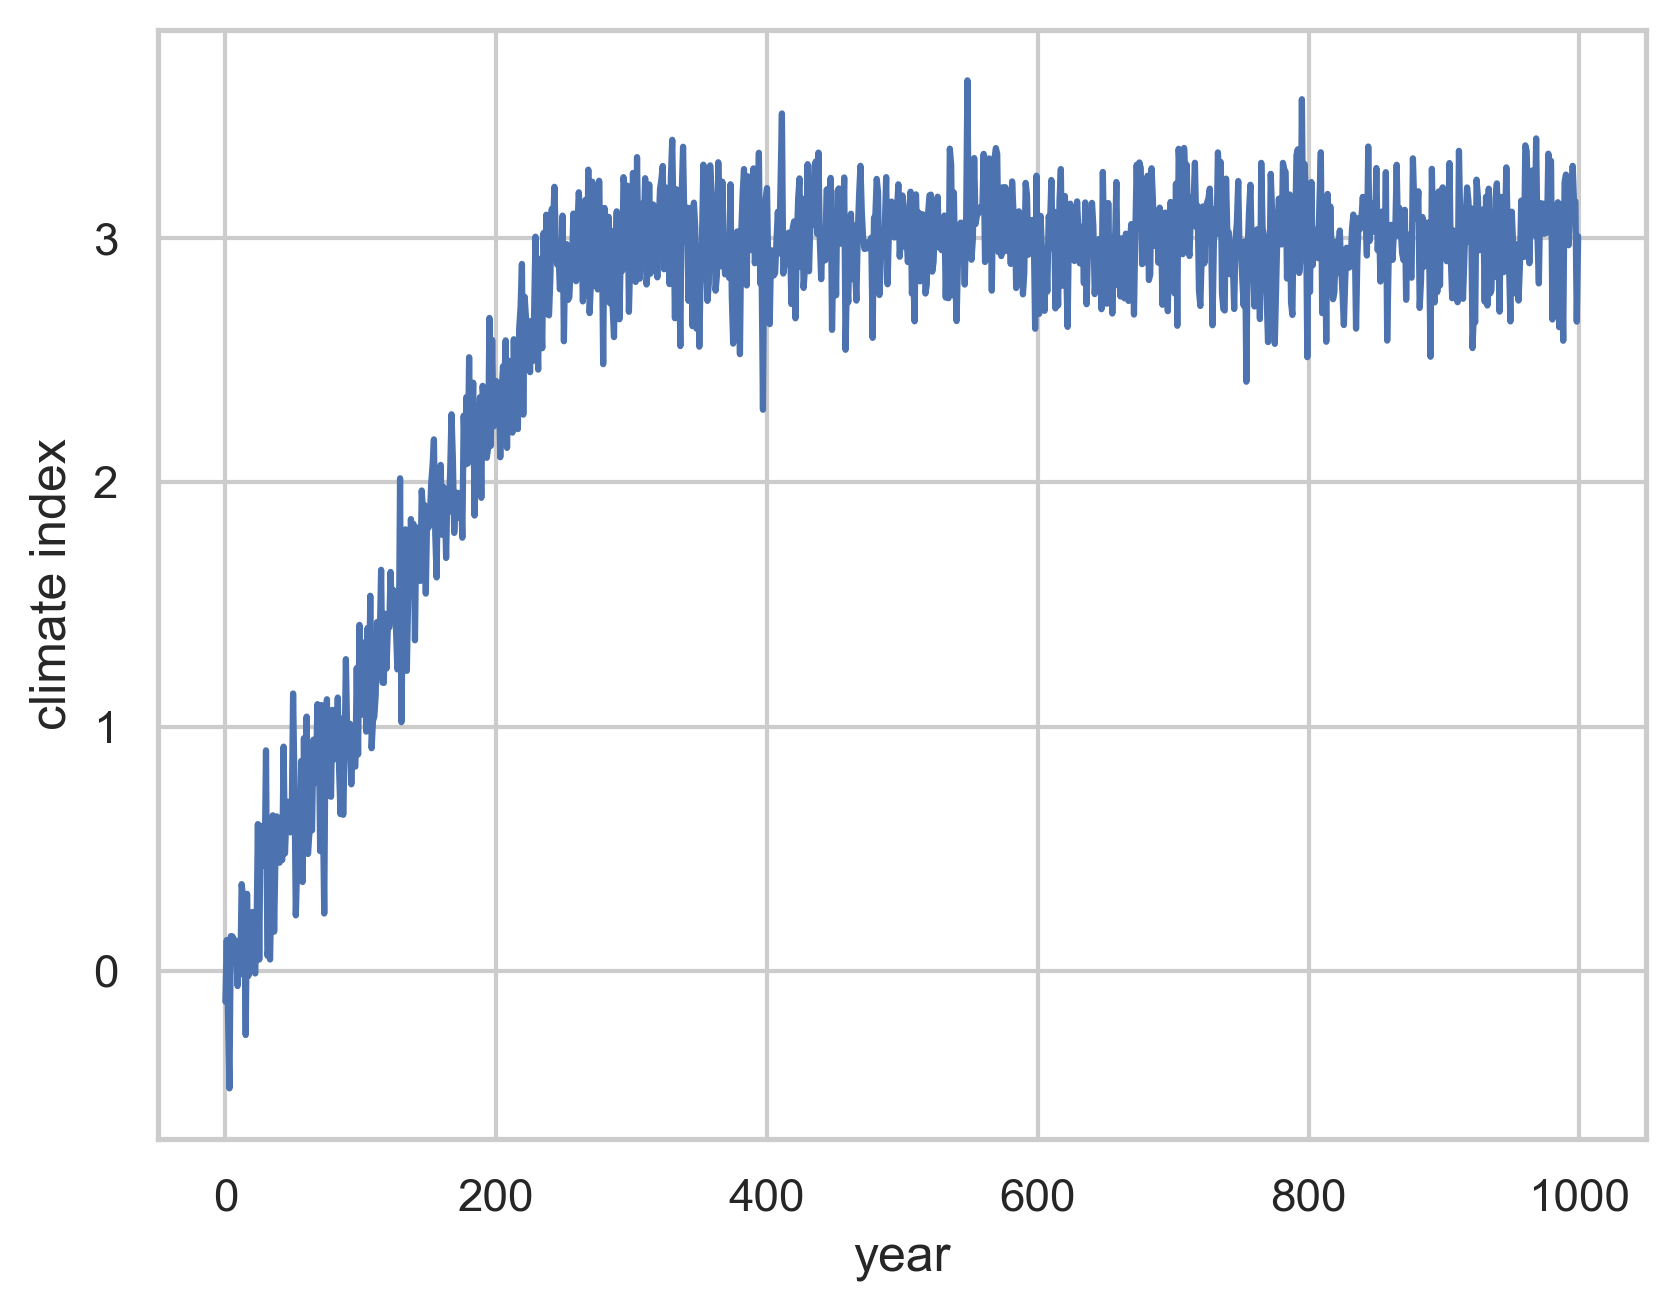
\includegraphics[width=0.6\textwidth]{../global-warming/figs/climate-index.png}
	\caption{The climate index spans \SI{1000}{\year}, and is provided as part of the glaciology course.}
	\label{fig:climate-index}
\end{figure}

\subsection{Idealized\_*}\label{app:forcing-idealized}

The idealized\_+12 forcing scenario is derived from an analysis of the climate index and the magnitude of the climate anomaly in 2100 CE, which is scaled by the climate index. Since the index peaks at \(\approx\num{3}\) and the temperature anomaly is \(\Delta T\approx\SI{4}{\celsius}\) (compare \cref{fig:era5,,fig:21c-warming}), increasing the temperature field by \(\Delta\mean{T}=\SI{12}{\celsius}\) yields a similar climate forcing as the NorESM case. Furthermore, \Textcite{greve2022} simulate the GrIS under a sustained late-21\textsuperscript{st}-century climate, hence, the temperature increase in the idealized\_+4 forcing is equal to the temperature anomaly in 2100 CE. This choice is within the projected window of global temperature rise in the RCP8.5, one of the pathways used by \textcite{greve2022}.

In both scenarios, changes in precipitation are neglected (\(\Delta P < \SI{0.2}{\mm\per\day}\)) and therefore computing of precipitation fields is unaltered.

\begin{figure}
	\centering
	\begin{subfigure}{0.46\textwidth}
		\centering
		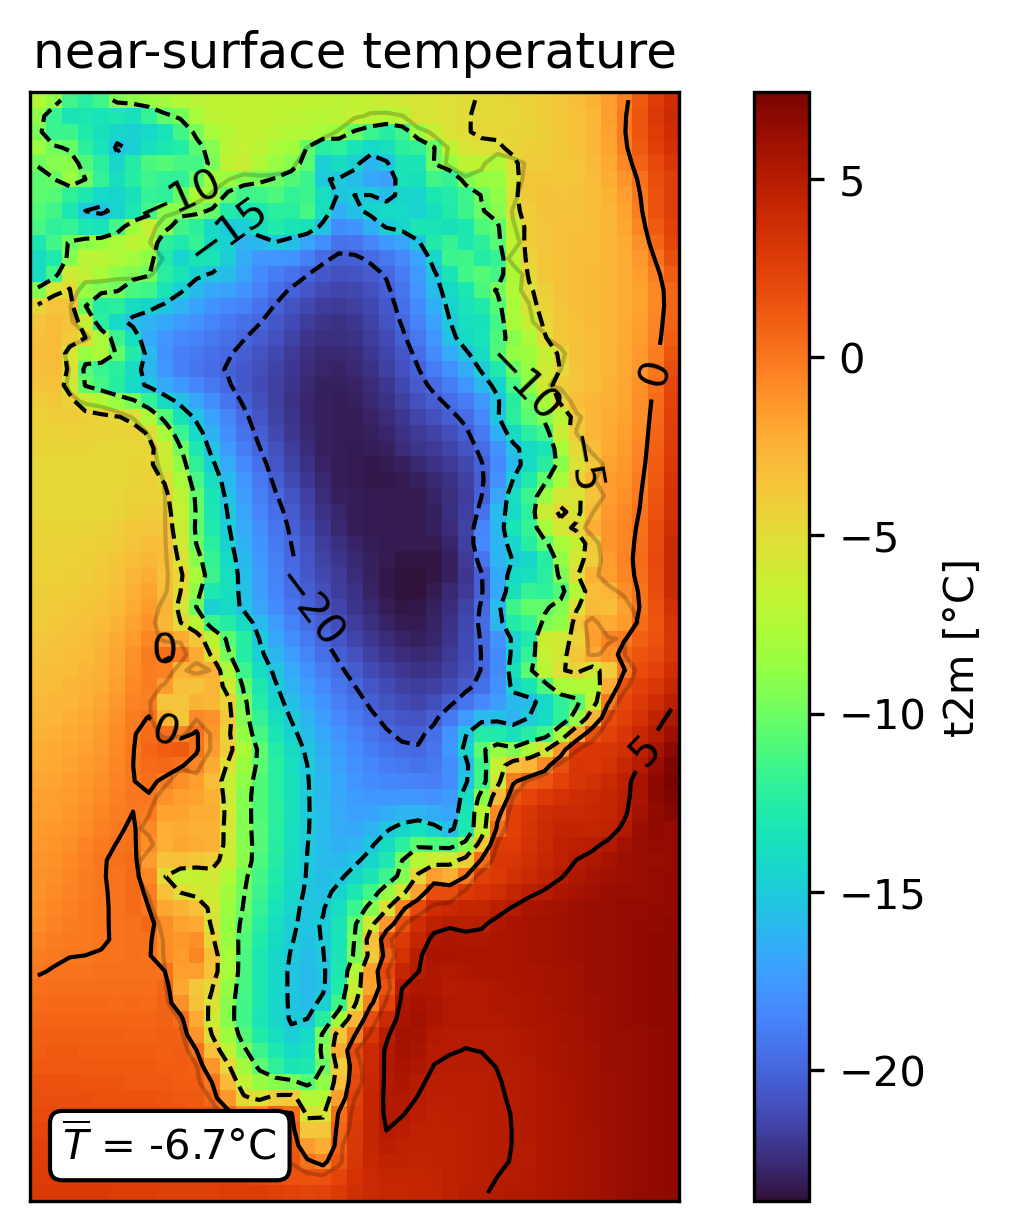
\includegraphics[width=\textwidth]{../global-warming/figs/21c-t2m-mean.png}
	\end{subfigure}
	\begin{subfigure}{0.44\textwidth}
		\centering
		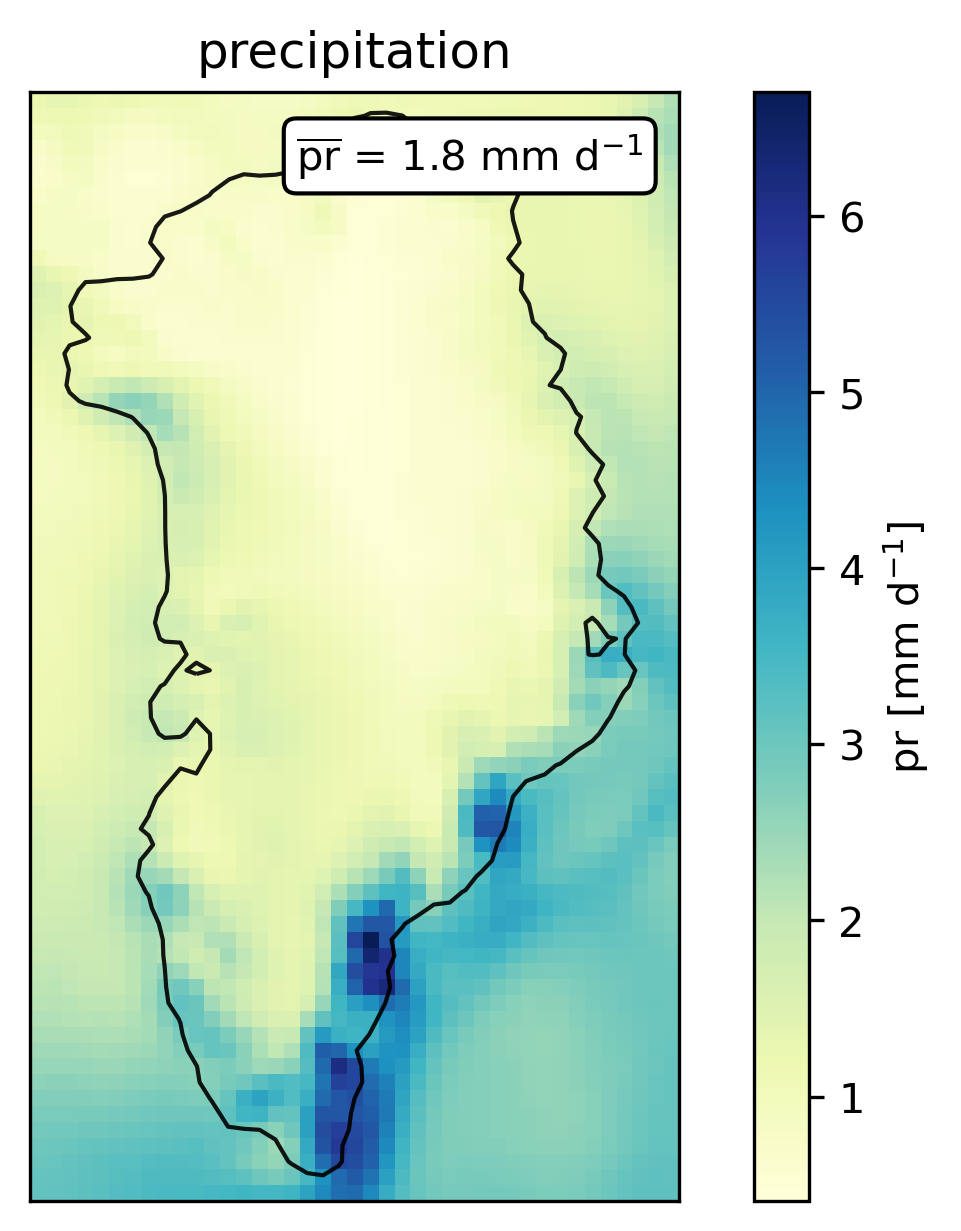
\includegraphics[width=\textwidth]{../global-warming/figs/21c-pr-mean.png}
	\end{subfigure}
	\caption{Annual mean near-surface temperature and precipitation for 2100 CE based on sum of projected anomalies by NorESM and present-day climatology}
	\label{fig:21c-warming}
\end{figure}

	
\end{document}